\documentclass{scrartcl}
\usepackage[english]{babel}
% deutsche Umlaute
\usepackage[utf8]{inputenc}
\usepackage[T1]{fontenc}
\usepackage{lmodern}

% für das H placement Kommando bei figures:
\usepackage{float}

\usepackage{graphicx}
\usepackage{varioref}
\usepackage[
bookmarks=true,	% Lesezeichen erzeugen
bookmarksopen=false,	% Lesezeichen ausgeklappt
bookmarksnumbered=true,	% Anzeige der Kapitelzahlen am Anfang der Namen der Lesezeichen
pdfstartpage=1,	% Seite, welche automatisch geöffnet werden soll
%baseurl=http://www.server.de/dateiname.pdf, 
%  URL des PDF-Dokuments (oder Hintergrundinformationen)
pdftitle={STAV Report},
% Titel des PDF-Dokuments
pdfauthor={Johannes Schneider, Tim Henning},	% Autor(Innen) des PDF-Dokuments
%pdfsubject={},	% Inhaltsbeschreibung des
%pdfkeywords={},
% Stichwortangabe zum PDF-Dokument
breaklinks=true,	% ermöglicht einen Umbruch von URLs
colorlinks=true,	% Einfärbung von Links
linkcolor=black,	% Linkfarbe: schwarz (z.B. im Inhaltsverzeichnis)
anchorcolor=blue,	% Ankerfarbe: schwarz
citecolor=black, % Literaturlinks: schwarz
filecolor=black,	% Links zu lokalen Dateien: schwarz
menucolor=black, % Acrobat Menü Einträge: schwarz
pagecolor=blue, % Links zu anderen Seiten im Text: schwarz
urlcolor=black,	%  URL-Farbe: schwarz
%backref=true,
pagebackref=false,
pdfcenterwindow=true,
pdfnewwindow=true,
pdffitwindow=true,
pdfstartview=FitH,
pdfpagemode=UseOutlines
]{hyperref}
\usepackage{cleveref}


\title{TAV - Report}
\subtitle{Project: Luminosus}
\author{Johannes Schneider and Tim Henning}

\begin{document}

\maketitle

\setcounter{section}{-1}
\section{Application Selection}

\subsection{Introduction}

Extending the functionality of a lighting desk can be a difficult and time consuming task. To make it more easy to integrate and test new features the idea was to create a separate modular software platform that is connected via network to the lighting console. As a solution for this "Luminosus" was developed.

\begin{figure}[h]
	\centering
	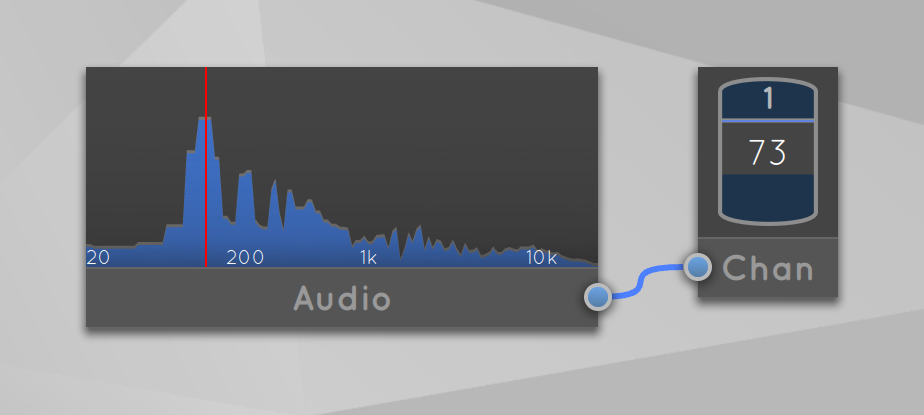
\includegraphics[width=0.5\textwidth]{img/luminosus_example}
	\caption[Luminosus Example]{Luminosus Example: Controlling the brightness of channel 73 by the current audio level}
	\label{fig:luminosus_example}
\end{figure}

The main project development was done by Tim Henning while writing his bachelor thesis. He is the only developer of the project till now. For this V\&V project Johannes Schneider joins the project as a developer and tester.

The programming language used is C++ 11 with syntax additions by Qt. The user interface part uses the descriptive language QML that includes function definitions in JavaScript.

The application is intended to be used by end users. It runs as a desktop application on Windows and MacOS and as an app on Android and iOS.

The existing code base consists of approximately 40k LOC (C++ source and header files + QML files).

Available artifacts are the source code, documentation, changelog, issue tracker, manual and in addition the Bachelor thesis \textit{Entwicklung einer modularen Benutzeroberfl\"ache als zus\"atzliche Bedieneinheit einer Lichtkonsole} including a requirement analysis and a discussion of the architectural decisions.

No specific development paradigm was used.

The current V\&V status is that only manual tests are performed (adding all available function blocks as a kind of 'smoke test' is available in the GUI) and static code analysis using Clang is provided by the IDE. Verification was not done yet.

\subsection{Learning from failures}

In the following section some random failures of the application shall be introduced and analyzed what can be learned from them.

\paragraph{Issue \href{https://github.com/ETCLabs/LuminosusEosEdition/issues/2}{\#2} Connection to Eos stopped working:}

After a while the network connection of the software to the lighting console stopped working. The user was not able to continue using the application for the show even after restarting everything.

While the fault is not yet known the issue is probably complexity related. Many different devices were involved and it is not clear whether the problem was caused by this software or a different failing part in the system.


\paragraph{Issue \href{https://github.com/ETCLabs/LuminosusEosEdition/issues/3}{\#3} Faders not updated:}

The user described an issue where the fader positions were not updated correctly after switching the page of faders.

The issue was caused by a single missing line of code that would reset the positions of all faders to 0 before requesting and setting the new positions.
Thus the issue can be categorized as preventable as the fault could have been found by unit tests that cover all branches of the code.


\paragraph{Issue \href{https://github.com/ETCLabs/LuminosusEosEdition/issues/4}{\#4} Fullscreen on iOS not working:}

The issues states that the fullscreen button is not working correctly on the iOS platform. The failure is visible as too large UI elements that render the application unusable after clicking on the fullscreen button.

On the one hand the fault can be categorized as preventable since it could be detected by a simple unit test that compares the scale property before and after the operation.
On the other hand it is also a type of intelligent fault since the real problem was the pure existence of a fullscreen button on a mobile operating system. So even if the function would have been working as expected, the resulting behavior would be irritating as the only difference of the fullscreen mode on a mobile OS is the removal of the status bar that is in this case not very useful.

\paragraph{Conclusion}
In general the introduction of unit tests would be a valuable addition to the existing code base. Furthermore integration tests for typical user scenarios would help to prevent many kind of faults. Last but not least we learned that to maintain so many different platforms the user feedback is an important part in the process of V\&V.


\subsection{Five Basic V\&V Questions}

\paragraph{When do V\&V start?  When are they complete?}

Validation started right in the beginning. The project was validated on a daily basis  due to a lot of contact to the supervisor. The specification was adjusted very frequently to ensure that the features that were developed were suitable for the projects goal.

Analysis began early, too, in the form of static code analysis provided by the IDE (Qt Creator) and CLang. The development of tests did not start till the begin of this V\&V project.

The process of V\&V does not end till the end of the lifetime of the product. In this case as long as the software is maintained.

\paragraph{What particular techniques should be applied during development?}

Static code analysis is very good applicable for C++ due to strict type declarations. 

Continuous Integration should be applied to the project since it will be used on various platforms. Furthermore automated unit testing will be applied during the semester.

Additionally profiling the memory consumption can help finding memory leaks and performance benchmarks make sure that the specification is met in terms of latency and responsibility.

In the end a formal verification of standardized components such as the network protocol implementations should be applied.

\paragraph{How can we asses the readiness of the product?}

The readiness is assessed by using the defined features of the specification and their current implementation status. Before a release is considered ready it should be at least tested manually in a typical use case scenario.

Furthermore open issues are a hint that the product is not yet ready.

In the end the validation of a product is easier when the developer is also a user like in our case. The greater the distance of the developer to the users of the product the harder it is to match the use cases with the implementation. 

\paragraph{How can we control the quality of successive releases?}

To ensure that successive releases do not introduce new faults a pre-release policy can be established to let a small group of beta users test the system before it is released to the public.

The successful run of automated tests, especially regression tests, in a Continuous Integration environment can be a good indicator, too.

\paragraph{How can the development process itself be improved?}

Increasing emphasis on applying various V\&V techniques during further development will help to improve overall code quality. 

Furthermore the development process can be improved by introducing a second developer to the project. Thus pair programming and code reviews can be established to help finding flaws. In addition maintaining the documentation will lead to a better process.


\section{Analysis}

\subsection{Human-based Static Analysis}

\paragraph{Peer Review}

During our peer review session we discovered different faults in our project as well as in the project of our partner group. Thus, the peer review helped us exchange thoughts about various faults not only within our group but also with members of our partners group. Therefore we used the peer review mainly to enhance communication and understanding of the code. Additionally, we fixed the faults we discovered thus improving the code quality. Main advantages of this kind of peer review is the fact, that every code snippet can be discussed directly with its author. This enables a very deep discussion about certain implementation decisions and also improved the overall code understanding by far. After just a short while we were even able to detect a misleading documentation for a certain implementation, although we never saw the code before. 

%% old content
\if(false) 
The peer review helped understanding the code because it was possible to discuss the reviewed code directly with the author.
We were able to improve the general code quality and comments by pointing out parts that were difficult to understand.

The previously known bugs were found and we could even find a case where the description of a method did not match its content.

A good peer review is organized a few days before so that everyone can get into the code. Therefore the discussion can start right away. It also helps to question even minor things so that the author can either explain his thoughts or comes to really think of it for the first time.
\fi

We organized our peer review sessions by picking suitable code snippets for each other. These snippets were supposed to be readable, even for someone who is not as deeply involved in the project or even the programming language at all. We then presented the selected code to the other group while also introducing the general project. Afterwards, we further increased our understanding by asking questions about unclear syntax or general questions about details within the code. Finally, we were able to discuss issues we found and tried to find suitable solutions.

In general, peer reviews can help to improve the product by selecting difficult code and talk about it in a very objective way. Thus, we do not need to play the blaming game and can just focus on finding and avoiding faults for future implementations. Additionally, it is very important to do this kind of analysis on a regular basis, so that the reviewed code is still manageable in size and difficulty. 

\paragraph{Tools}

%% old content
\if(false)
A tool that is well suited for human-based peer reviews is the review function of GitHub (see \vref{fig:github_review_comment}). It allows for example to mark persons which have to review a pull request before it can be merged. Comments can be made for each line of code individually and the author can respond to them directly. It can also integrate various different tools and incorporate dynamical tests of continuous integration system like Travis CI, too.
\fi

A tool we are very comfortable using is GitHub. GitHub does not only allow you to host git repositories, so all your code is in just one place, but also offers a great variety of reviewing tools like commenting coding line by line (see \vref{fig:github_review_comment}). The concept of pull requests and its support is also a very strong feature in GitHub. It offers developers a very formal way of merging branches into each other. It supports a human based review process by naming one or more reviewers for the pull requests. These reviewers may then comment, ask questions or suggest improvements for the code at hand. Although this process is mostly covered by the features offered by GitHub, we would like to have a way of (autonomously) selecting code of interest as we did in our peer review. Right now, every reviewer has to read all the code submitted for merging, making it very time consuming.

\begin{figure}[h]
	\centering
	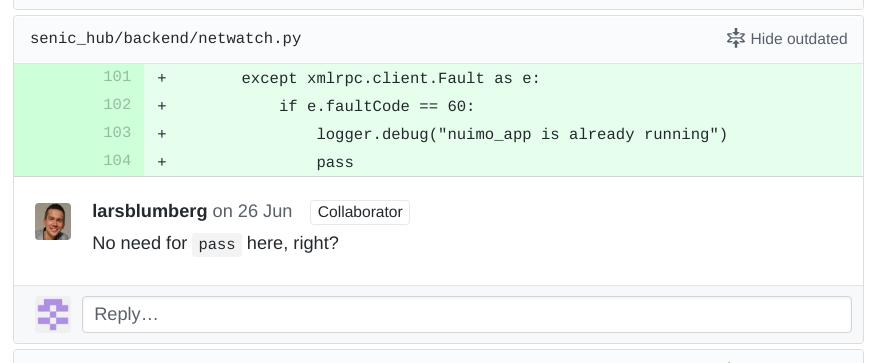
\includegraphics[width=0.9\textwidth]{img/github_review_comment}
	\caption[GitHub Review Comment]{A comment in the GitHub review tool}
	\label{fig:github_review_comment}
\end{figure}

While it is comfortable for the team members that these functions are integrated into the GitHub website and work in every browser, this means that no code exploration features known from various IDEs are available. As a beginning it would be nice for example to be able to jump to a function declaration right from the review page of GitHub. It would help the code understanding a lot.

Besides GitHub, SonarQube is another excellent web based tool for reviewing code. In contrast to GitHub, SonarQube is not used as a repository host. What makes SonarQube still great is its build-in fault detection and static analysis. Thus, a reviewer can find any flaws very fast and also see, who authored the corresponding code. We will cover more of the automated static analysis feature of SonarQube in section \ref{sec:humand-based-vs-automated-sa}.

\subsection{Automated Static Analysis}

\paragraph{Evaluation of Tools}

%% old content
\if(false)
We used Clang Static Analyzer and CppCheck for this project.
Both tools are well suited for C++ code and are supported by the IDE (Qt Creator). The detected faults are intuitively shown next to the corresponding line in the code.
\fi

In order to test automated static analysis we used the Clang Static Analyzer and CppCheck for our project. We chose these tools not only because they offer great plugins for the IDE of our choice (Qt Creator) but also because they are made for analyzing C++ code. Any detected fault is displayed directly in the code editor, next to the line where it is caused. 

On the one hand Clang helped to improve the code by finding a possible nullpointer dereference caused by a missing return statement. On the other hand it reported hundreds of false alarms in its default configuration, i.e. increase of precision of floating point numbers such making it harder to detect the real faults (see \vref{fig:clang_fp_implicit_precision_increase}).

Other than Clang, CppCheck found not initialized member variables. But even while it was designed not to show false positives, many of them were shown due to bugs in CppCheck (see \vref{fig:cppcheck_fp_missing_ctor}).

\begin{figure}[h]
	\centering
	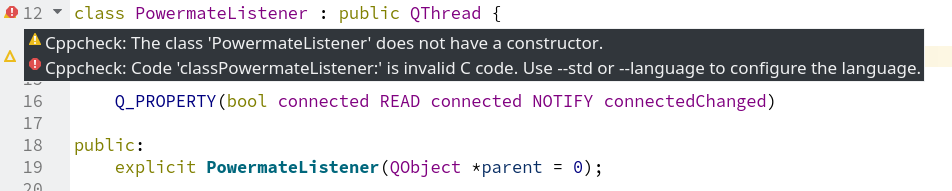
\includegraphics[width=0.9\textwidth]{img/cppcheck_fp_missing_ctor}
	\caption[Bugs in CppCheck]{Bugs in CppCheck result in false positives}
	\label{fig:cppcheck_fp_missing_ctor}
\end{figure}

Due to the heavy use of C++ in security critical environments there are many non-free tools for bug finding and formal validation it, too. An example for this is Polyspace that even claims to be able to proof the absence of some types of faults, such as buffer overflows, division by zero and wrong array accesses.

In the preparation of this report we tried to apply this tool to our project, but experienced some problems in using it (see \vref{fig:polyspace_analysis}). We were only able to validate one single source file, the only file with no dependencies other than the C++ standard library. To resolve the Qt includes it would be necessary to monitor the build process of the project by Polyspace, which was not possible due to a specific missing compiler on the system.

\begin{figure}[h]
	\centering
	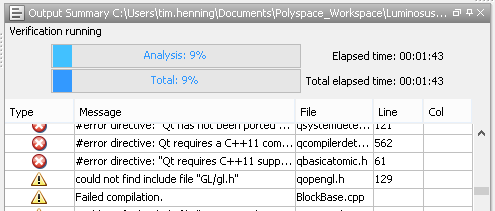
\includegraphics[width=0.7\textwidth]{img/polyspace_analysis}
	\caption[Polyspace Analysis]{Polyspace showing errors while analyzing C++ code with Qt dependencies}
	\label{fig:polyspace_analysis}
\end{figure}

\paragraph{Type of Inaccuracy}

While investigating the design and philosophy of the Clang static analyzer the developers clearly stated that the tool was made to reported as less false positives as possible. However, they are more concerned about not finding a fault, so they would tolerate a moderate amount of false alarms. This leaves us with the conclusion that the Clang static analyzer is mainly incorporating pessimistic inaccuracy, which results in false alarms. However, the tool can be configured to also include optimistic inaccuracy if needed. This can be realized by adding filters so that some checks will become less strict. This behavior will result in some faults not being detected any longer.

\begin{figure}[h]
	\centering
	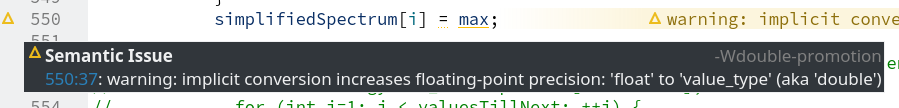
\includegraphics[width=0.9\textwidth]{img/clang_fp_implicit_precision_increase}
	\caption[Clang warns of increase in precision]{Clang warns of increase in precision of floating point number}
	\label{fig:clang_fp_implicit_precision_increase}
\end{figure}

According to their website, the goal of CppCheck is to have zero false positives, resulting in a low pessimistic inaccuracy. They even recommend to use an additional tool that has a greater pessimistic inaccuracy if required for the project. Unfortunately in practice there are still some false positive mainly related to bugs in CppCheck as already mentioned before. The developers state that there are many faults that are not detected by CppCheck which leads to a high optimistic inaccuracy.

This shows that trying to show as few false positives as possible often also implies that the user has to live with optimistic inaccuracy and that it is intended that not all faults are detected. Those tools can therefore not guarantee the absence of faults.

Polyspace is the only tool that we evaluated that claims to have zero optimistic inaccuracy for some kind of faults. It realizes this by abstract interpretation of the code and automated formal validation methods.

\subsection{Interaction between Human-Based and Automated SA}
\label{sec:humand-based-vs-automated-sa}

\begin{figure}[h]
	\centering
	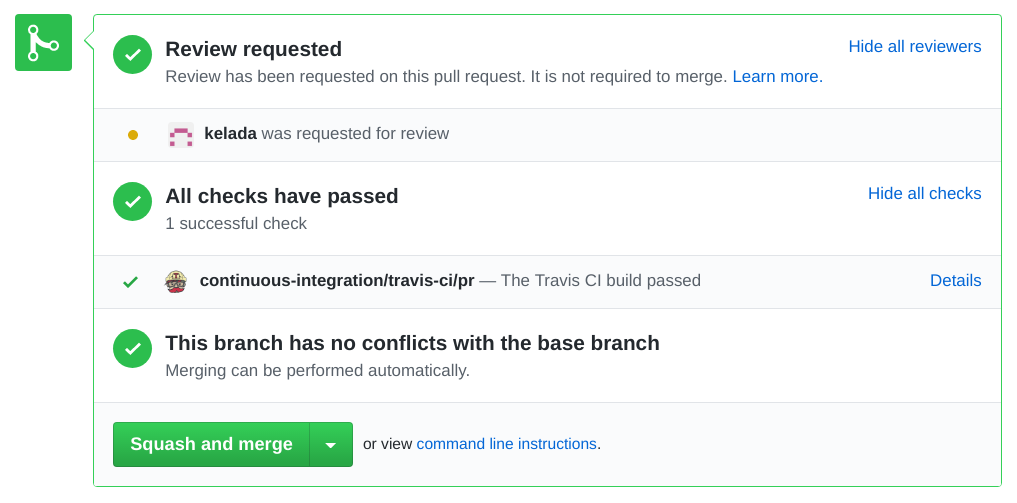
\includegraphics[width=0.9\textwidth]{img/github_pr_review}
	\caption[GitHub PR review]{Combination of ASA and human-based reviews in GitHub}
	\label{fig:github_pr_review}
\end{figure}

By using ASA a peer review can be prepared in order to point out potentially broken code parts. It can then be discussed if a detected fault is considered a false positive or not and how to fix it. Additionally, some faults might be caused by a bad habit within the project team. These faults are very interesting to discover and can indicate certain lacks of the developing team, enabling more overall awareness once discussed thoroughly. They might even cause a change in the general consideration of good code in the team.  

When using tools like SonarQube, the faults get matched with their author. This enables each developer to learn from their mistakes in a more direct way. Additionally it also displays which kind of faults are often produced in a project. These faults can then be targeted by further education and more awareness.

When thinking the other way around, the results of a human-based peer review can be used to improve the configuration of the automated static analysis tools. This can reduce the number of false positives which are caused by the coding guidelines of the individual project and thus are intended.
Depending on the use case, the relevance of faults is differently prioritized. In our specific case the implicit increase of precision of floating point numbers is not a problem at all. In contrast, in more space critical applications this could lead to unpredictable behavior.

In addition to the combination of ASA and human-based reviews, testing can also be integrated in this process. GitHub is a good example for this, as it shows the result of different software verification and validation methods at one glance as seen in \vref{fig:github_pr_review}.

\end{document}
